\documentclass[a4paper, 12pt]{article}
\usepackage[hidelinks]{hyperref}
\usepackage{graphicx}
\graphicspath{ {images/} }
\begin{document}
\title{Requirements Documentation for SCSS Student Forum}
\author{Group 2 - Screw you Gary we'll call it what we want}
\maketitle
	\section{Introduction}
		\subsection{Overview}
			\begin{itemize}
				\item Our project aims to create a forum for students of 
				Computer Science to use to be able to discuss different topics 
				and matters regarding to the course, and to be able to give 
				and receive help from their course mates.
				\item Currently, a platform suitable for discussion 
				of computer science coursework is conspicuously missing. 
				If a student is confused about an assignment, they may 
				contact the tutor or the professor, or their course friends, 
				all of whom may not be able or willing to help at all. 
				We propose a better solution, one where you can gather more 
				responses from your course mates, and are able to contribute 
				to others who face similar problems and can achieve them 
				together, A Computer Science dedicated forum.
			\end{itemize}
		\subsection{Scope}
			\begin{itemize}
				\item We wish to have a single forum that encompasses all modules 
				for all year groups across Integrated Computer Science, Computer 
				Science and Business, and Computer Science and a Language. Users should be able to:
				\begin{itemize}
					
					\item Post new topics in each module page.
					\item Reply to existing topic threads.
					\item Choose best response to the current thread.
				\end{itemize}
				\item The forum should only be accessible to students, demonstrators, 
				teaching assistants and lecturers with a valid @tcd.ie email address.
			\end{itemize}
		\subsection{Objectives and Success Criteria}
			\begin{itemize}
				\item To complete the forum by Week 10 of Hilary Term.
				\item To host the forum on the Trinity KDEG servers, which we have been given access to. 
				The forum should handle multiple users at a time and should accept each valid email to sign up.
				\item To program the front end in HTML/PHP and design a back end SQL database.
				\item To communicate with our expected user base, which are the student body 
				associated with SCSS, in order to ensure that the forum meets their expectations, 
				and to guarantee the forum would be something they would use once it is made available.
			\end{itemize}
		\subsection{Definitions, Abbreviations}
			\begin{itemize}
				
				\item SCSS - School of Computer Science and Statistics.
				\item CS - Computer Science.
				\item CSB - Computer Science and Business.
				\item CSL - Computer Science and a Language.
				\item HTML - HyperText Markup Language.
				\begin{itemize}
					\item Used as standard markup language in creating websites.
				\end{itemize}
				\item PHP - Personal Home Page.
				\begin{itemize}
					\item Used for web design and also as a general purpose programming language.
				\end{itemize}
				\item Forum - An online discussion site where people can hold conversations in the
				form of posted messages.
				\item UI - User Interface.
			\end{itemize}
			\subsection{References}
			\begin{itemize}
				\item \url{http://www.vbulletin.com/forum/help?faq=vb3_board_usage#faq_vb3_forums_threads_posts}
				\item \url{http://php.net/manual/en/preface.php}
			\end{itemize}
	\newpage
	\section{Proposed System}
		\subsection{Overview}
			\begin{itemize}
				\item An online forum where students of CS, CSB, and CSL can discuss course topics 
				and trade opinions, ideas and feedback. The forum will allow users to create new topic 
				threads, reply to existing topics and choose the best response to the topic they created. 
				\item The moderators of the forum will be given tools to manage the overall forum. They will 
				be able to delete threads they deem inappropriate, remove spam/derogatory posts and remove users. 
				This will all be manageable using SQL permissions.
			\end{itemize}
		\subsection{Functional Requirements}
			\begin{itemize}
				\item The forum in its final state should:
				\begin{itemize}
					\item Store unique usernames
					\begin{itemize}
						\item Each user should have a unique username based off of their Trinity email.
					\end{itemize}
					\item Allow creation of new threads
					\begin{itemize}
						\item Each user should have permission to create a new topic of discussion.
						\item Users should be able to create replies to this discussion.
					\end{itemize}
					\item Choose best response to a topic
					\begin{itemize}
						\item Users that create topics should be able to highlight the reply that they received the 
						most help or information from in general so other users with similar complaints can also see it.	
					\end{itemize}
				\end{itemize}
			\end{itemize}
		\subsection{Non-functional Requirements}
			\begin{itemize}
				\item The forum should prioritize:
				\begin{itemize}
					\item Scalability
					\begin{itemize}
						\item The forum should remain efficient and swift regardless of number of threads and users.
					\end{itemize}
					\item Efficiency
					\begin{itemize}
						\item The forum should be efficient and responsive i.e a forum post should appear immediately,
						pages should load instantaneously etc.
					\end{itemize}
					\item Security
					\begin{itemize}
						\item The forum will keep user information secure via passwords and unique IDs.
					\end{itemize}
				\end{itemize}
			\end{itemize}
		\subsection{System Prototype}
			\begin{itemize}
				\item UI Mockups \\
				\vspace{10 mm}
				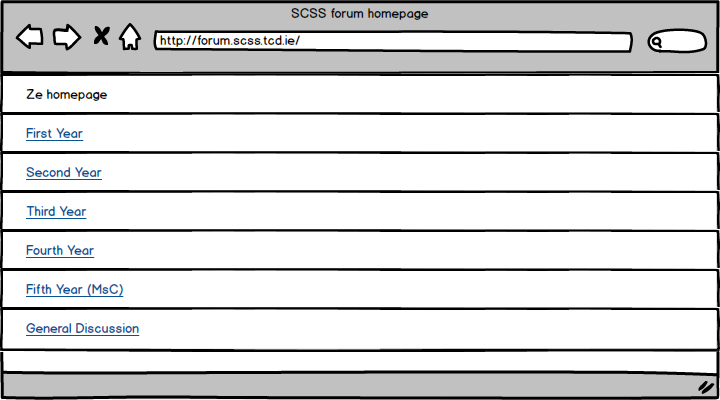
\includegraphics[width=\textwidth]{homepage}
				\vspace{10 mm}
				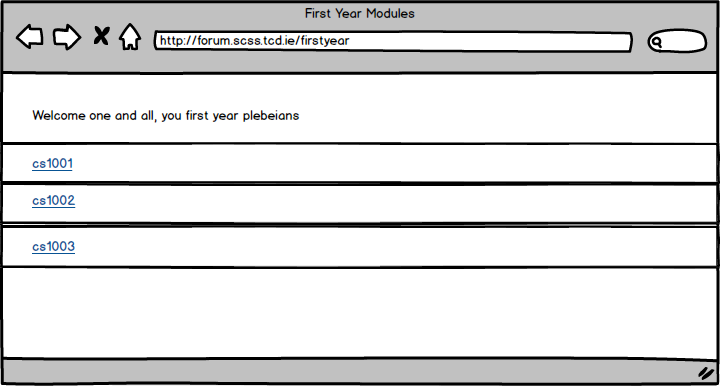
\includegraphics[width=\textwidth]{yearPage}
				\vspace{10 mm}
				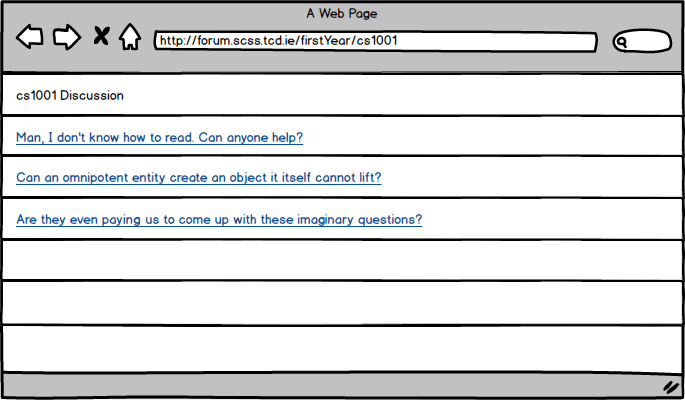
\includegraphics[width=\textwidth]{coursePage}
				\vspace{10 mm}
				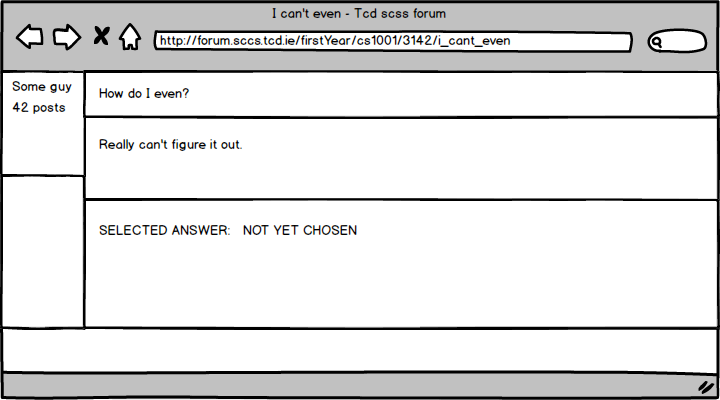
\includegraphics[width=\textwidth]{thread}
				\vspace{10 mm}
				\newpage
				\item UML Use Case Diagram \\
				\vspace{10 mm}
				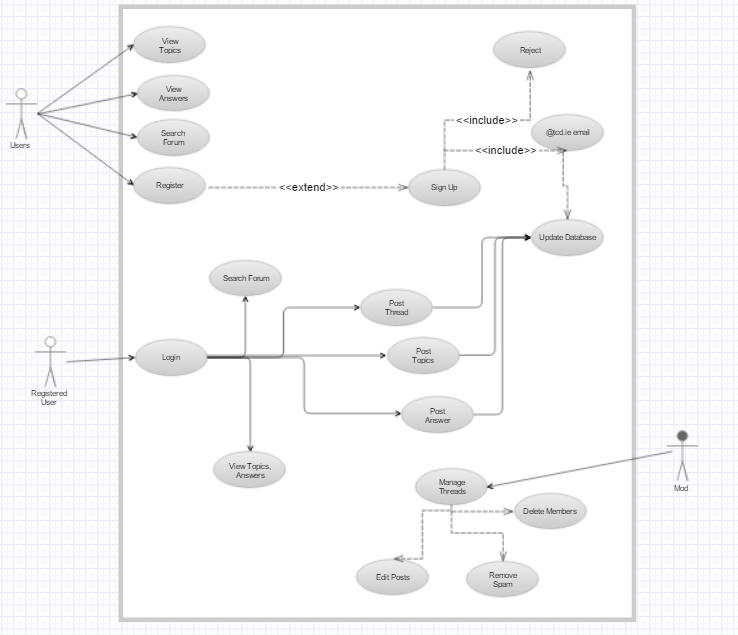
\includegraphics[width=\textwidth]{usecase}
			\end{itemize}


\end{document}
